	\pagestyle{fancy}
	
	\section{Theoretische Grundlagen} \label{sec:Theoretische Grundlagen}
	
	\subsection{Grundlagen der Finite-Elemente-Methode}\label{sec:Grundlagen-FEM}
	Die Finite-Elemente-Methode (FEM) ist eine zuverlässige und weitverbreitete numerische Analysemethode. Dabei wird hauptsächlich die lineare Finite-Elemente-Methode verwendet, aufgrund ihrer einfachen Anwendung in vielen Bereichen.\\
	
	Die Grundidee der Finite-Elemente-Methode besteht darin, den kontinuierlichen Lösungsbereich in eine Gruppe von finiten Einheiten zu diskretisieren, die auf bestimmte Weise miteinander verbunden sind. Die Unterteilung der ganzen Lösungsbereich in einfachere Teile hat mehrere Vorteile:
	\begin{itemize}
		\item Darstellung von komplexen Geometrien,
		\item Einbeziehung unterschiedlicher Materialeigenschaften,
		\item Einfache Darstellung der Gesamtlösung,
		\item Erfassung von lokalen Auswirkungen.
	\end{itemize}

	Da die Elemente verschieden kombiniert und selbst unterschiedliche Formen haben können, ist es möglich, eine Lösungsdomäne mit komplexen geometrischen Formen zu modellieren. Ein weiteres wichtiges Merkmal der Finite-Elemente-Methode ist die Verwendung von angenommenen Näherungsfunktionen, um die unbekannte Feldfunktion darzustellen, die in der vollständigen Lösungsdomäne gesucht wird. Die Näherungsfunktion im Element wird normalerweise durch den Wert der unbekannten Feldfunktion oder ihre Ableitung an jedem Knoten des Elements und ihre Interpolationsfunktion ausgedrückt. Auf diese Weise wird der Wert der unbekannten Feldfunktion oder ihrer Ableitung an jedem Knoten zur Unbekannten (d.h. zum Freiheitsgrad). Damit wird ein kontinuierliches Problem mit unendlich vielen Freiheitsgraden  zu einem diskreten Problem mit endlich vielen Freiheitsgraden umgesetzt \cite{schwarz2013methode}. \\
	
	Sobald die Unbekannten bestimmt sind, kann der Näherungswert der Feldfunktion in jedem Element durch die Interpolationsfunktion berechnet werden, um die Näherungslösung in der gesamten Lösungsdomäne zu erhalten. Offensichtlich nimmt die Genauigkeit der Lösung weiter zu, wenn die Anzahl der Elemente zunimmt oder wenn die Freiheitsgrade je Element zunehmen. Wenn das Element die Konvergenzanforderungen erfüllt, konvergiert die Näherungslösung schließlich zur exakten Lösung \cite{kattan2010matlab}.
	
	\subsubsection{Nichtlineare Finite-Element-Berechnungen}\label{sec:n.lin_FEM}
	Im Wesentlichen sind alle Probleme der Festkörpermechanik nichtlinear, und es gibt nur wenige analytische Lösungen. Probleme der linearen elastischen Mechanik sind nur eine vereinfachte Annahme der praktischen Probleme. Bei der Finite-Elemente-Analyse umfassen die Annahmen der Linearisierung normalerweise Folgendes:
	\begin{enumerate}
		\item die Knotenverschiebung ist ein kleiner Betrag;
		\item das Material ist linear elastisch;
		\item die Eigenschaften der Randbedingungen sind unverändert während der Bewegung oder Verformung des Körpers.
	\end{enumerate}
	Wenn eine der oben genannten drei Annahmen nicht erfüllt ist, handelt es sich um ein nichtlineares Problem.
	In Anbetracht dessen werden nichtlineare Probleme in der Festkörpermechanik im Allgemeinen in drei Kategorien unterteilt, nämlich Materialnichtlinearität, geometrische Nichtlinearität und Nichtlinearität der Randbedingungen.
	
	\subsubsection{Geometrische Nichtlinearität}\label{sec:geo-n.lin}
	Geometrisch nichtlineare Probleme beziehen sich häufig auf große Verschiebungen oder große Dehnungen innerhalb der Struktur.  Ein Sonderproblem stellen große Verschiebung (wie Translation oder Rotation) mit gleichzeitig kleinen Dehnung dar \cite{rust2011nichtlineare}. In dieser Arbeit dreht der Werkzeugschaft mit hoher Rotationsgeschwindigkeit und Exzentrizität, wodurch nichtlineare Verzerrungen  (nach Green-Lagrange) berücksichtigt werden. Das Materialverhalten soll jedoch als linear elastisch angenommen werden \\
	
	\begin{figure}[H]
		\centering
		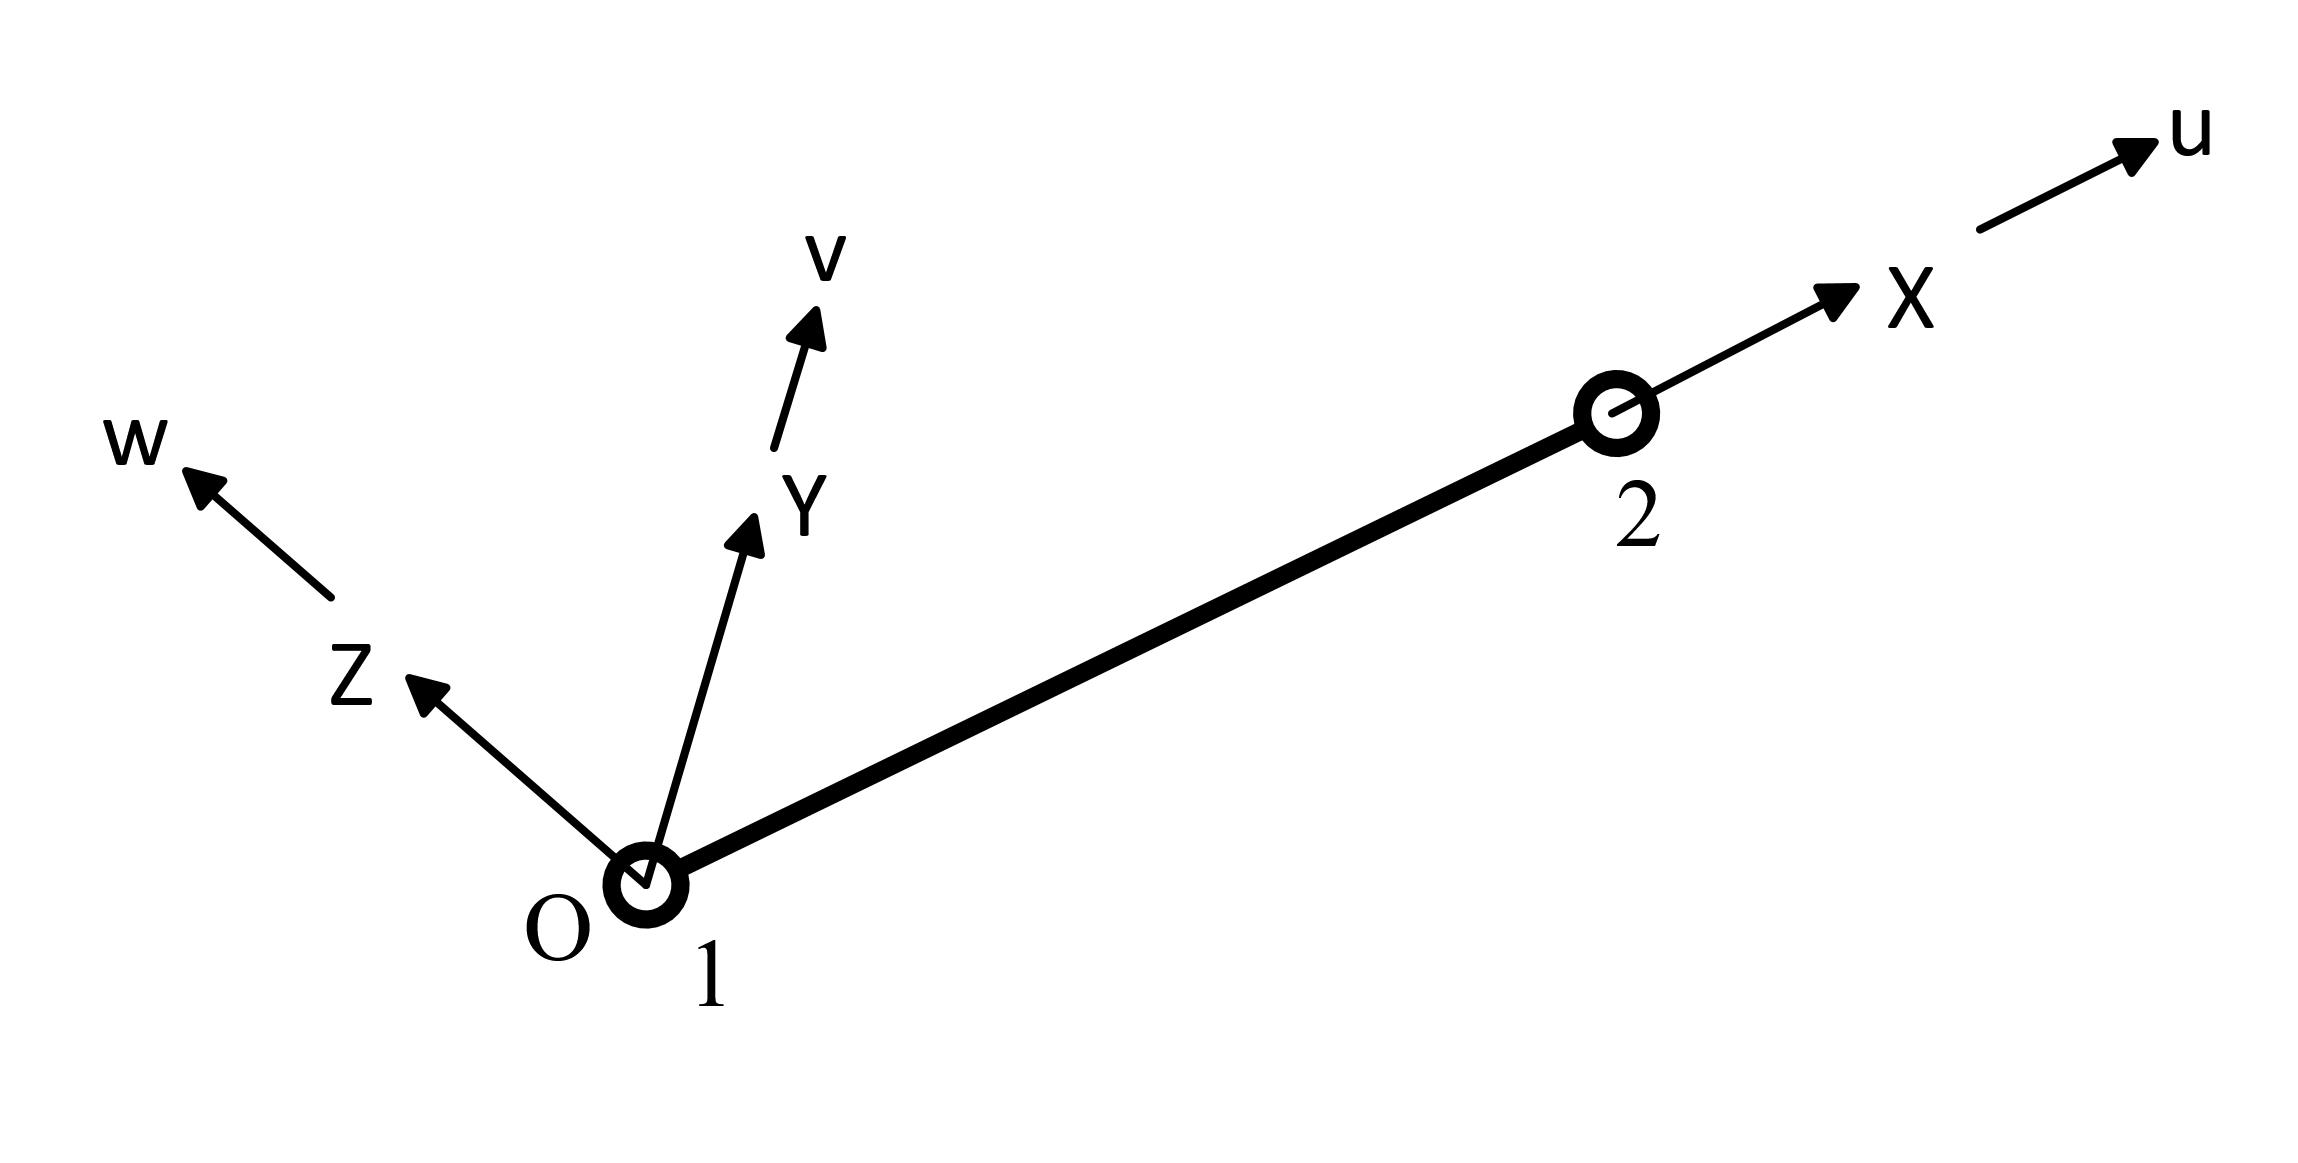
\includegraphics[width=0.74\linewidth, height=0.23\textheight]{Theoretische_Grundlagen/2_Knote_Element}
		\caption{Zweiknotiges Balkenelement mit Koordinaten und Verschiebungen.}
		\label{fig:2-Knote-Element-Koordinate}
	\end{figure}
	
	In Abbildung \ref{fig:2-Knote-Element-Koordinate} ist ein zweiknotiges Balkenelement dargestellt. Weiterhin sind die Verschiebungen $ u $, $ v $ und $ w $ eingetragen. Dabei ist $ u $ die Längsverschiebung und $ v $ sowie $ w $ die Durchbiegungen. Die Green-Lagrange-Dehnungen basieren auf der Änderung des Abstands zwischen zwei benachbarten Punkten. Die genannte Veränderung des Balkens (verformte Länge $ l $, unverformte Länge $ l_{0} $) kann mit
	
	\begin{equation}\label{equ:Änderung der Quadrate}
	\begin{aligned}
	\Delta & = \frac{l^{2}-l_{0}^{2}}{l_{0}^{2}} = \frac{(l_{0}+u)^{2}+v^{2}+w^{2}-l_{0}^{2}}{l_{0}^{2}} = \frac{l_{0}^{2}+2l_{0}u+u^{2}+v^{2}+w^{2}-l_{0}^{2}}{l_{0}^{2}} \\
	       & = 2\frac{u}{l_{0}}+\left(\frac{u}{l_{0}}\right)^{2}+\left(\frac{v}{l_{0}}\right)^{2}+\left(\frac{w}{l_{0}}\right)^{2} .
	\end{aligned}
	\end{equation}
	
	beschrieben werden. Beim Übertragung zum finiten Element ergibt sich
	
	\begin{equation}\label{equ:Übergang zum dx bei Dehnung}
	\frac{u}{l_{0}} \rightarrow \frac{\partial u}{\partial x}=u_{x} \quad \mathrm{;} \quad \frac{v}{l_{0}} \rightarrow \frac{\partial v}{\partial x} = v_{x} \quad \mathrm{;}  \quad \frac{w}{l_{0}} \rightarrow \frac{\partial w}{\partial x}=w_{x}
	\end{equation}
	
	und deshalb
	
	\begin{equation}\label{equ:2.-Änderung der Quadrate}
	\Delta = 2 \frac{\partial u}{\partial x} + \left( \frac{\partial u}{\partial x} \right)^{2} + \left( \frac{\partial v}{\partial x} \right)^{2} + \left( \frac{\partial w}{\partial x} \right)^{2} .
	\end{equation}
	
	Für kleine Verformungen ist das Quadrat vernachlässigbar, sodass nur der erste Term erhalten bleibt, der doppelt so hoch ist wie die lineare oder mechanische Dehnung. Deswegen wird die Green-Lagrange-Dehnung in X-Richtung durch die Hälfte der Änderung der Quadrate gegeben:
	
	\begin{equation}\label{equ:Green-Lagrange-Dehnung}
	\varepsilon_{GL} = \frac{\Delta}{2} = \frac{\partial u}{\partial x} + \frac{1}{2} \left( \frac{\partial u}{\partial x} \right)^{2} + \frac{1}{2} \left( \frac{\partial v}{\partial x} \right)^{2} +\frac{1}{2} \left( \frac{\partial w}{\partial x} \right)^{2} = u_{x}+ \frac{1}{2} u_{x}^{2} + \frac{1}{2} v_{x}^{2} + \frac{1}{2} w_{x}^{2} .
	\end{equation}
	
	\subsection{Lösung nichtlinearer Gleichungssysteme}\label{sec:Lösungsverfahren-n.lin_Dgl}
	
	Für die Finite-Elemente-Methode werden die Knotenverschiebungen als unbekannt Grundparameter verwendet. Das mechanische Modell wird im Allgemeinen nach der Finite-Elemente-Diskreti\-sierung, Elementanalyse, Systemgruppierung und Einführung von Randbedingungen in der Form
	
	\begin{equation}\label{equ:Bewegung-GL}
	\mathbf{M}\, \ddot{\vec{x}}+ \mathbf{D}\, \dot{\vec{x}}+ \mathbf{K}\, \vec{x} = \vec{f} \ ,
	\end{equation}
	
	dargestellt. Dabei ist $ \vec{x} $ der unbekannte Knotenverschiebungsvektor und $ \vec{f} $ der äquivalenter Knotenkraftvektor. Sowohl $ \vec{x} $ und $ \vec{f} $ besitzen die Ordnung $n$. $ \mathbf{M} $ , $ \mathbf{D} $ und $ \mathbf{K} $ sind die Massen-, Dämpfungs- und Steifigkeitsmatrix des Systems. Die Steifigkeitsmatrix ist im Allgemeinen eine positiv definite Matrix. \\
	
	Für statische Probleme kann die Gleichung (\ref{equ:Bewegung-GL}) wie folgt
	
	\begin{equation}\label{equ:Einfach-Bewegung-GL}
	\mathbf{K}\, \vec{x} = \vec{f}
	\end{equation}
	
	vereinfacht werden. Bei dynamischen Problemen müssen zusätzlich die Anfangsbedingungen
	
	\begin{equation}\label{equ:Anfangsbedingung-Bewegung-GL}
	\begin{array}{cc}
	\vec{x}|_{t=0}=\vec{x}_{0} & \dot{\vec{x}}|_{t=0}=\dot{\vec{x}}_{0}
	\end{array}
	\end{equation}
	
	für Gleichung (\ref{equ:Bewegung-GL}) beachtet werden.\\
	
	Wenn $ \mathbf{K} $ oder $\vec{f}$ eine Funktion von $ \vec{x} $ und (oder) dessen Zeitableitung ist, dann wird das Problem nichtlinear. Normalerweise können die nichtlineare Gleichungen nicht direkt gelöst werden. Sie können durch eine Reihe linearer algebraischer Gleichungen angenähert werden, sodass das Lösungsverfahren komplizierter und zeitaufwendiger ist. Es gibt viele Linearisierungsmethoden, z.B. \textsc{Newton}-\textsc{Raphson}-Verfahren \cite{rust2011nichtlineare}, Quasi-\textsc{Newton}-Verfahren \cite{luenberger1984linear}, Modifiziert-\textsc{Newton}-Verfahren, das BFGS-Verfahren und das DFP-Verfahren \cite{matthies1979solution}. In dieser Arbeit wird \textsc{Newton}-\textsc{Raphson}-Verfahren benutzt.\\
	
	Das \textsc{Newton}-\textsc{Raphson}-Verfahren wird mechanisch als Tangentensteifigkeitsmethode bezeichnet und ist eine der bekanntesten Methoden zur Lösung der nichtlinearen Gleichungen. Zur Vereinfachung der Beschreibung kann die Gleichung (\ref{equ:Einfach-Bewegung-GL}) wie folgt umgeschrieben werden:
	
	\begin{equation}\label{equ:Newton-Vereinfach-Bewegung-GL}
	\vec{\varPsi}(\vec{x}) = \mathbf{K}(\vec{x}) \cdot \vec{x}-\vec{f}=\vec{0} \ .
	\end{equation}
	
	Dabei ist $ \vec{\varPsi} $ eine stetige ableitbare Funktion mit dem Näherungsanfangsvektor $ \vec{x}^{(0)} $ und dem Näherungsvektor nach der $n$-ten Iteration ist $ \vec{x}^{(n)} $. Nach der Taylorreihenentwicklung von $ \vec{\varPsi} $ werden die linearen Terme beibehaltet und die Terme höheren Ordnung ignoriert, sodass sich
	
	\begin{equation}\label{equ:Taylorreihe-Newton-Vereinfach-Bewegung-GL}
	\vec{\varPsi}(\vec{x}^{(n)}) = \mathbf{K}_{\text{T}}^{(n)} (\vec{x}-\vec{x}^{(n)})\approx 0
	\end{equation}
	
	ergibt. Mit der Lösung aus Gleichung (\ref{equ:Taylorreihe-Newton-Vereinfach-Bewegung-GL}) kann ein neuer Näherungsvektor mit
	
	\begin{equation}\label{equ:Naeherungswert-x(n+1)}
	\vec{x}^{(n+1)} = \vec{x}^{(n)} - \left( \mathbf{K}_{\text{T}}^{(n)} \right)^{-1} \cdot \vec{\varPsi}(\vec{x}^{(n)}) \ .
	\end{equation}
	
	 berechnet werden. Tie Tangentensteifigkeitsmatrix der Struktur
	
	\begin{equation}\label{equ:Taylorreihe-K}
	\mathbf{K}_{\text{T}}^{(n)} = \left. \dfrac{\partial \vec{\varPsi}}{\partial \vec{x}}\right| _{\vec{x}=\vec{x}^{(n)}}
	\end{equation}
	
	 besteht aus einem Zusammenbau der Tangentensteifigkeitsmatrizen der entsprechenden Elemente. Durch Vergleichen des relativen Fehlers mit dem Ergebnis des vorherigen Iterationsschritts kann der Konvergenzprozess gesteuert werden.\\
	 
	 Deshalb kann der Lösungsmethode von \textsc{Newton}-\textsc{Raphson}-Verfahren bei Programmierung mit folgender Schritte beschreiben:
	 \begin{enumerate}
	 	\item Anfangswert $ x^{(0)} $ und $ n=0 $ einstellen,
	 	\item Tangentensteifigkeitsmatrizen $ \mathbf{K}_{\text{T}}^{(n)} $ berechnen:
	 	\begin{equation}\label{equ:Tangentensteifigkeitsmatrizen}
	 	\mathbf{K}_{\text{T}}^{(n)} = \left. \dfrac{\partial \vec{\varPsi}}{\partial \vec{x}}\right| _{\vec{x}=\vec{x}^{(n)}} ,
	 	\end{equation}
	 	\item $ \vec{\varPsi}^{(n)} $ berechnen:
	 	\begin{equation}\label{equ:Psi-Berechnen}
	 	\vec{\varPsi}^{(n)} = \vec{\varPsi}(\vec{x}^{(n)}) = \mathbf{K}(\vec{x}^{(n)}) \vec{x}^{(n)}-\vec{f},
	 	\end{equation}
	 	\item Funktion $ \mathbf{K}_{\text{T}}^{(n)} \Delta \vec{x}^{(n)} = -\vec{\varPsi}^{(n)} $ lösen und bekommen:
	 	\begin{equation}\label{equ:Delta-X}
	 	\Delta\vec{x}^{(n)} = - (\mathbf{K}_{\text{T}}^{(n)})^{-1} \vec{\varPsi}^{(n)},
	 	\end{equation}
	 	\item neuer Näherungsvektor berechnen:
	 	\begin{equation}\label{equ:Naeherungswert-(n+1)}
	 	\vec{x}^{(n+1)} = \vec{x}^{(n)} + \Delta\vec{x}^{(n)},
	 	\end{equation}
	 	\item Wenn es konvergiert, endet die Iteration; andernfalls lassen $ n=n+1 $ und noch mit Schritt 2 fortfahren.
	 \end{enumerate}
	 
	 \subsection{Prinzip von Hamilton} \label{sec:prinzip-hamilton}
	 In der Physik ist das Prinzip von \textsc{Hamilton} der Ausdruck des 1833 vom irischen Physiker \textsc{William Hamilton} veröffentlichten Prinzips. Das Prinzip von \textsc{Hamilton} besagt, dass die Dynamik eines physikalischen Systems mittels Variationsrechnung einer einzigen Funktion, der \textsc{Lagrange}-Funktion welche alle physikalischen Informationen über das System und die darauf einwirkenden Kräfte enthält, bestimmt wird. \\
	 
	 Für ein System mit potentieller und kinetischer Energie lautet die \textsc{Lagrange}-Funktion nach \cite{gross2004technische}
	 \begin{equation}\label{equ:lagrange-funktion}
	 L = E_{kin} - E_{pot}.
	 \end{equation}

	 
	 Das Hamilton-Prinzip bietet die Möglichkeit, die Bewegung physikalischer Systeme auszudrücken. Anders als die Differentialgleichungsmethode des \textsc{Newton}'schen Bewegungsgesetzes verwendet diese Methode ein Funktional in Form eines  Zeitintegrals.\\
	 
	 Das Prinzip von \textsc{Hamilton} ist auch ein wichtiges Variationsprinzip in der Elastodynamik. Im Gegensatz zu einem System, das aus starren Körper besteht, haben verformbare Körper unendlich viele Freiheitsgrade. Der Zustand des Systems wird daher durch kontinuierliche Funktionen von Raum und Zeit beschrieben. Das erweiterte Prinzip von \textsc{Hamilton} für solche Körper wird durch
	 \begin{equation}\label{equ:Hamilton}
	 \delta\int_{t_{1}}^{t_{2}} \left( E_{kin}-E_{pot}\right)  \mathrm{d}t + \int_{t_{1}}^{t_{2}} \delta W \mathrm{d}t = 0
	 \end{equation}
	 gegeben.
	 Nacheinander sind also die kinetische Energie $ E_{kin} $ und die potenzielle Energie $ E_{pot} $ des Systems sowie die virtuelle Arbeit $ \delta W $ aller angreifenden potentiallosen Kräfte zu bestimmen \cite{wauer2014kontinuumsschwingungen}.
	 
